\begin{figure}
  \centering
  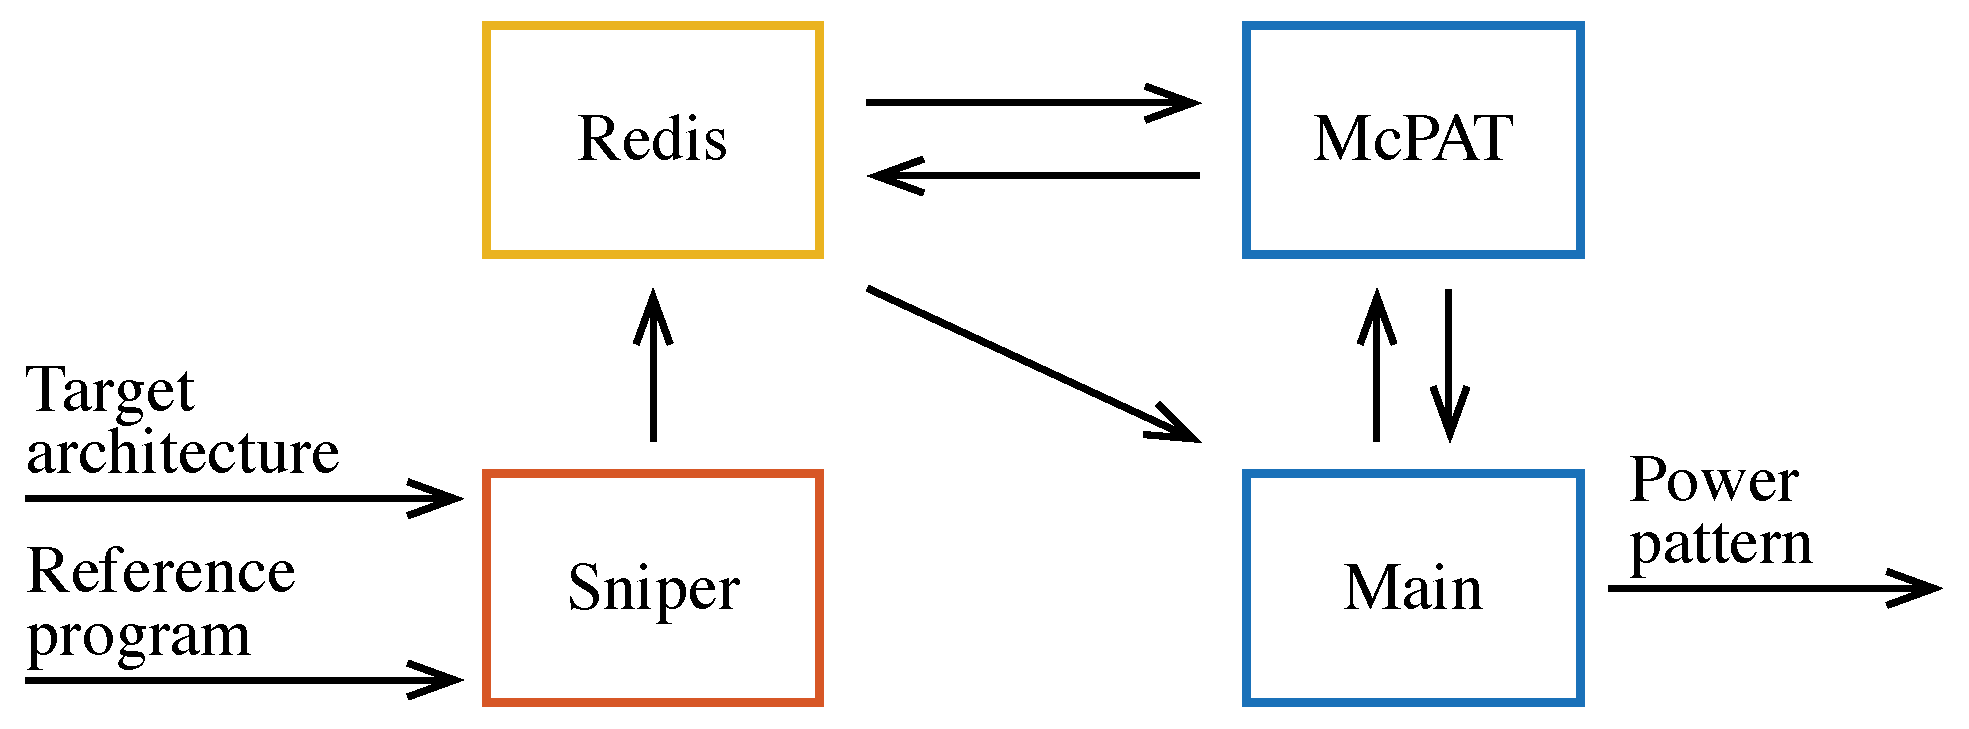
\includegraphics[width=1.0\columnwidth]{include/assets/figures/recorder.pdf}
  \caption{
    The recording infrastructure. The Recorder tool corresponds to the two blue
    boxes on the right-hand side of the figure.
  }
  \flab{recorder}
\end{figure}

The Recorder tool is used at the data-acquisition stage of our methodology in
order to record reference workload patterns, which are discussed in
\sref{workload} and needed for Streamer. In \fref{methodology}, Recorder
corresponds to the bottom-left boxes labeled ``Recorder.'' The tool has a
curtain infrastructure around it. This infrastructure is depicted in
\fref{recorder}, in which Recorder itself is represented by the two blue boxes
on the right-hand side.

Given a reference application and a target platform, the first step is
performance simulation, which we undertake by virtue of the Sniper simulator
\cite{carlson2011}. The output of the simulator is a series of files containing
performance-related information over time. These files are further processed by
our Recorder.

The communications between Sniper and Recorder are handled by Redis \cite{redis}
(see \fref{recorder}), which is an in-memory key-value storage commonly used for
caching and message passing. Whenever Sniper produces a new file with
performance information, it sends a message with the file's location to a Redis
queue. Recorder fetches this message from the queue (observe the diagonal arrow
in \fref{recorder}) and processes the corresponding file. There are several
aspects to note here. First, the indirection allows Sniper and Recorder to work
asynchronously, each at its own pace. Second, there can be multiple Recorder
processes serving the same message queue. Third, there can be many Sniper
processes, each of which simulates a different program and uses a different
Redis queue. The above aspects substantially seed up the recording.

The next step is power simulation, which is delegated to \sc{McPAT}
\cite{li2009}. \sc{McPAT} is originally a command-line program; we have made a
shared library out of it and embedded it into Recorder. In addition, we have
introduced a caching mechanism into \sc{McPAT}, which is inspired by Sniper. The
caching mechanism eliminates the repetition of certain computations inside
\sc{McPAT}, which leads to considerable time savings. For caching purposes, we
again use Redis; see the direct arrows between Redis and \sc{McPAT} in
\fref{recorder}. All Recorder processes that are connected to the same Redis
server can leverage the same cache, making the caching mechanism shine.

Finally, the computed power pattern is stored in a file, which can then be
uploaded to a repository, as described in \sref{workload} and illustrated in
\fref{methodology}. Each such output file is an SQLite database \cite{sqlite},
which implies that the versatile SQL language is automatically at one's disposal
for working with the data.
